\documentclass{article}
%----------------------------------------------------------------------------------------
%	PACKAGES AND OTHER DOCUMENT CONFIGURATIONS
%----------------------------------------------------------------------------------------

\usepackage{amsmath,amsfonts,stmaryrd,amssymb} % Math packages

\usepackage{enumerate} % Custom item numbers for enumerations
\usepackage{tikz}
\usetikzlibrary{arrows}
\usepackage[ruled]{algorithm2e} % Algorithms

\usepackage[framemethod=tikz]{mdframed} % Allows defining custom boxed/framed environments

\usepackage{listings} % File listings, with syntax highlighting
\lstset{
	basicstyle=\ttfamily, % Typeset listings in monospace font
}

%----------------------------------------------------------------------------------------
%	DOCUMENT MARGINS
%----------------------------------------------------------------------------------------

\usepackage{geometry} % Required for adjusting page dimensions and margins
\usepackage{graphicx, amsmath, amsthm, amssymb, listings, multirow, wrapfig, floatrow}
\newcommand{\bigCI}{\mathrel{\text{\scalebox{1.07}{$\perp\mkern-10mu\perp$}}}}
\usepackage{xepersian}
\settextfont[Scale=1]{XB Niloofar}
\setdigitfont[Scale=1]{Yas}

\geometry{
	paper=a4paper, % Paper size, change to letterpaper for US letter size
	top=2.5cm, % Top margin
	bottom=3cm, % Bottom margin
	left=2.5cm, % Left margin
	right=2.5cm, % Right margin
	headheight=14pt, % Header height
	footskip=1.5cm, % Space from the bottom margin to the baseline of the footer
	headsep=1.2cm, % Space from the top margin to the baseline of the header
	%showframe, % Uncomment to show how the type block is set on the page
}

%----------------------------------------------------------------------------------------
%	COMMAND LINE ENVIRONMENT
%----------------------------------------------------------------------------------------

% Usage:
% \begin{commandline}
%	\begin{verbatim}
%		$ ls
%		
%		Applications	Desktop	...
%	\end{verbatim}
% \end{commandline}

\mdfdefinestyle{commandline}{
	leftmargin=10pt,
	rightmargin=10pt,
	innerleftmargin=15pt,
	middlelinecolor=black!50!white,
	middlelinewidth=2pt,
	frametitlerule=false,
	backgroundcolor=black!5!white,
	frametitle={Command Line},
	frametitlefont={\normalfont\sffamily\color{white}\hspace{-1em}},
	frametitlebackgroundcolor=black!50!white,
	nobreak,
}

% Define a custom environment for command-line snapshots
\newenvironment{commandline}{
	\medskip
	\begin{mdframed}[style=commandline]
}{
	\end{mdframed}
	\medskip
}

%----------------------------------------------------------------------------------------
%	FILE CONTENTS ENVIRONMENT
%----------------------------------------------------------------------------------------

% Usage:
% \begin{file}[optional filename, defaults to "File"]
%	File contents, for example, with a listings environment
% \end{file}

\mdfdefinestyle{file}{
	innertopmargin=1.6\baselineskip,
	innerbottommargin=0.8\baselineskip,
	topline=false, bottomline=false,
	leftline=false, rightline=false,
	leftmargin=2cm,
	rightmargin=2cm,
	singleextra={%
		\draw[fill=black!10!white](P)++(0,-1.2em)rectangle(P-|O);
		\node[anchor=north west]
		at(P-|O){\ttfamily\mdfilename};
		%
		\def\l{3em}
		\draw(O-|P)++(-\l,0)--++(\l,\l)--(P)--(P-|O)--(O)--cycle;
		\draw(O-|P)++(-\l,0)--++(0,\l)--++(\l,0);
	},
	nobreak,
}

% Define a custom environment for file contents
\newenvironment{file}[1][File]{ % Set the default filename to "File"
	\medskip
	\newcommand{\mdfilename}{#1}
	\begin{mdframed}[style=file]
}{
	\end{mdframed}
	\medskip
}

%----------------------------------------------------------------------------------------
%	NUMBERED QUESTIONS ENVIRONMENT
%----------------------------------------------------------------------------------------

% Usage:
% \begin{question}[optional title]
%	Question contents
% \end{question}

\mdfdefinestyle{question}{
	innertopmargin=1.2\baselineskip,
	innerbottommargin=0.8\baselineskip,
	roundcorner=5pt,
	nobreak,
	singleextra={%
		\draw(P-|O)node[xshift=1em,anchor=west,fill=white,draw,rounded corners=5pt]{%
		Question \theQuestion\questionTitle};
	},
}

\newcounter{Question} % Stores the current question number that gets iterated with each new question

% Define a custom environment for numbered questions
\newenvironment{question}[1][\unskip]{
	\bigskip
	\stepcounter{Question}
	\newcommand{\questionTitle}{~#1}
	\begin{mdframed}[style=question]
}{
	\end{mdframed}
	\medskip
}

%----------------------------------------------------------------------------------------
%	WARNING TEXT ENVIRONMENT
%----------------------------------------------------------------------------------------

% Usage:
% \begin{warn}[optional title, defaults to "Warning:"]
%	Contents
% \end{warn}

\mdfdefinestyle{warning}{
	topline=false, bottomline=false,
	leftline=false, rightline=false,
	nobreak,
	singleextra={%
		\draw(P-|O)++(-0.5em,0)node(tmp1){};
		\draw(P-|O)++(0.5em,0)node(tmp2){};
		\fill[black,rotate around={45:(P-|O)}](tmp1)rectangle(tmp2);
		\node at(P-|O){\color{white}\scriptsize\bf !};
		\draw[very thick](P-|O)++(0,-1em)--(O);%--(O-|P);
	}
}

% Define a custom environment for warning text
\newenvironment{warn}[1][Warning:]{ % Set the default warning to "Warning:"
	\medskip
	\begin{mdframed}[style=warning]
		\noindent{\textbf{#1}}
}{
	\end{mdframed}
}

%----------------------------------------------------------------------------------------
%	INFORMATION ENVIRONMENT
%----------------------------------------------------------------------------------------

% Usage:
% \begin{info}[optional title, defaults to "Info:"]
% 	contents
% 	\end{info}

\mdfdefinestyle{info}{%
	topline=false, bottomline=false,
	leftline=false, rightline=false,
	nobreak,
	singleextra={%
		\fill[black](P-|O)circle[radius=0.4em];
		\node at(P-|O){\color{white}\scriptsize\bf i};
		\draw[very thick](P-|O)++(0,-0.8em)--(O);%--(O-|P);
	}
}

% Define a custom environment for information
\newenvironment{info}[1][Info:]{ % Set the default title to "Info:"
	\medskip
	\begin{mdframed}[style=info]
		\noindent{\textbf{#1}}
}{
	\end{mdframed}
}
 
\title{تمرین کامپیوتری سوم - استنتاج علّی} 
\author{بهراد منیری\\95109564\\ \texttt{bemoniri@live.com}}
\date{دانشکده‌ی مهندسی برق - دانشگاه صنعتی شریف}
%----------------------------------------------------------------------------------------

\begin{document}
\maketitle
\begin{center}
\begin{Large}\textbf{ 
 پیاده‌سازی الگوریتم شمارش تعداد اعضای هر کلاس هم‌ارزی مارکوف
}
\end{Large}
\end{center}


در این تمرین الگوریتم مطرح شده در 
\cite{count}
را در پایتون به کمک کتاب‌خانه‌‌ی
\lr{networkx}
پیاده‌سازی می‌کنیم. 
\section{
تابع
	chainCom}
این تابع
\lr{UCCG}
و یک گره از آن‌را در ورودی گرفته و خروجی آن گراف اساسی (\lr{CPDAG}) ای است که از روت قرار دادن گره داده‌شده به‌دست می‌آید. این تابع همچنین تمام
\lr{Chain Component}
های گراف ساخته شده را نیز خروجی می‌دهد.

برای آزمودن صحت پیاده‌سازی الگوریتم، از مثال بخش 
\lr{3.2.1}
 مقاله‌ی 
\cite{count}
استفاده می‌کنیم. شکل 
\eqref{fig1}
 یک گراف 
 \lr{UCCG}
 و تمام 
 \lr{v-rooted essential graph}
 ‌های آن را نشان می‌دهد.
\begin{figure}[h!]
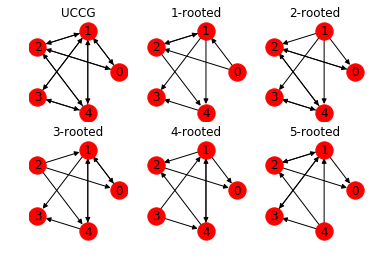
\includegraphics[scale=0.9]{chains.png}
\caption{خروجی الگوریتم‌ برای مثال مقاله‌ی
\cite{count}	
}
\label{fig1}
\end{figure}
خروجی مطابق نتایجی است که در خود مقاله مطرح شده است.

\section{تابع 
\lr{sizeMEC}
}
این تابع در ورودی یک گراف 
\lr{UCCG}
را می‌گیرد. هر 
\lr{UCCG}
نمایش‌دهنده‌ی یک کلاس هم‌ارزی مارکوفی است. این تابع در خروجی تعداد اعضای گراف هم‌ارزی مارکوف مربوط به 
\lr{UCCG}
داده‌شده را در خروجی برمی‌گرداند. (لطفاً تابع
\lr{adjCountMEC}
و 
\lr{CountMEC}
را نیز ببینید.)
در این‌ بخش نیز مثال مطرح شده در 
\cite{count}
را بررسی می‌کنیم. این گراف در شکل 
\eqref{fig1}
رسم شده است.
\textbf{ خروجی الگوریتم‌ ما عدد ۱۴ است که همان نتیجه‌ی مقاله است.}

\section{تابع
\lr{randomDAG}
}
این تابع در ورودی خود تعداد راس‌های مطلوب و احتمال وجود هر بال را گرفته و در خروجی یک 
\lr{DAG}
تصادفی با ویژگی‌های یادشده را  بر می‌گرداند. 
\section{تابع
\lr{dag2cpdag}
}
این تابع یک 
\lr{DAG}
را در ورودی گرفته و در خروجی یک 
\lr{CPDAG}
بر می‌گرداند. قواعد 
\lr{Meek}
در این تابع پیاده‌سازی شده‌اند.

شکل 
\eqref{fig2}
نمونه‌ای از اجرای این الگوریتم است.
\begin{figure}[h!]
	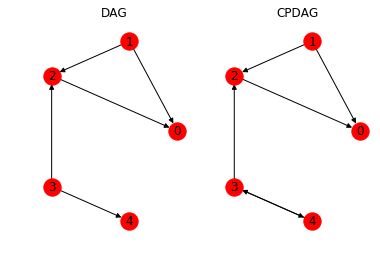
\includegraphics[scale=0.6]{meek.png}
	\caption{به دست آوردن گراف اساسی یک گراف جهت‌دار بدون دور}
	\label{fig2}
\end{figure}

\section{تابع 
	\lr{CountMEC}
}
این تابع بر خلاف توابع قبل که یک گراف 
\lr{UCCG}
می‌گرفتند، یک 
\lr{CPDAG}
در ورودی گرفته و تعداد اعضای کلاس هم ارزی مربوط به آن را برمی‌گرداند. 

\textbf{
برای تست کردن این تابع، تعداد اعضای کلاس هم‌ارزی گراف شکل \eqref{fig1} و شکل \eqref{fig2} را به دست می‌آوریم. این تابع به درستی برای گراف \eqref{fig1} عدد ۱۴  و برای گراف \eqref{fig2} عدد ۲ را باز می‌گرداند.}

\section{تابع 
	\lr{adjCountMEC}
}
این تابع کاملاً مشابه تابع 
\lr{CountMEC}
است با این تفاوت که در ورودی، ماتریس مجاورت گراف را می‌گیرد.

\section{در ادامه}
زنجیره‌ی مارکوف مقاله‌ی 
\cite{mcmc}
\newpage
\bibliographystyle{acm-fa}
\bibliography{bib}
\end{document}